%%%%%%%%%%%%%%%%%%%%%%% file template.tex %%%%%%%%%%%%%%%%%%%%%%%%%
%
% This is a general template file for the LaTeX package SVJour3
% for Springer journals.          Springer Heidelberg 2010/09/16
%
% Copy it to a new file with a new name and use it as the basis
% for your article. Delete % signs as needed.
%
% This template includes a few options for different layouts and
% content for various journals. Please consult a previous issue of
% your journal as needed.
%
%%%%%%%%%%%%%%%%%%%%%%%%%%%%%%%%%%%%%%%%%%%%%%%%%%%%%%%%%%%%%%%%%%%
%
% First comes an example EPS file -- just ignore it and
% proceed on the \documentclass line
% your LaTeX will extract the file if required
%
\RequirePackage{fix-cm}
%
%\documentclass{svjour3}                     % onecolumn (standard format)
%\documentclass[smallcondensed]{svjour3}     % onecolumn (ditto)
\documentclass[smallextended]{svjour3}       % onecolumn (second format)
%\documentclass[twocolumn]{svjour3}          % twocolumn
%
\smartqed  % flush right qed marks, e.g. at end of proof
%
\usepackage{amsmath}
\usepackage{booktabs}
\usepackage{subcaption}
\usepackage{tabularx}
\usepackage{nicefrac}
\usepackage[usenames]{xcolor}
\usepackage{lineno,hyperref}
\usepackage{graphicx}
%
% \usepackage{mathptmx}      % use Times fonts if available on your TeX system
%
% insert here the call for the packages your document requires
%\usepackage{latexsym}
% etc.
%
% please place your own definitions here and don't use \def but
% \newcommand{}{}
%
% Insert the name of "your journal" with
% \journalname{myjournal}
%
\begin{document}

\title{Formation of transverse cracks from the growth of multiple adjacent debonds on consecutive fibers in UD composites under transverse tension: Effect of the mutual position of debonds on Energy Release Rate
}
%\subtitle{}

%\titlerunning{Short form of title}        % if too long for running head

\author{Luca Di Stasio   \and
        Janis Varna \and
        Zoubir Ayadi
}

%\authorrunning{Short form of author list} % if too long for running head

\institute{Luca Di Stasio \at
              Lule\aa\ University of Technology, University Campus, SE-97187 Lule\aa, Sweden\\
              Universit\'e de Lorraine, EEIGM, IJL, 6 Rue Bastien Lepage, F-54010 Nancy, France\\
              \email{luca.di.stasio@ltu.se}           %  \\
%             \emph{Present address:} of F. Author  %  if needed
           \and
           Janis Varna \at
              Lule\aa\ University of Technology, University Campus, SE-97187 Lule\aa, Sweden\\
              \email{janis.varna@ltu.se}
		\and
           Zoubir Ayadi \at
              Universit\'e de Lorraine, EEIGM, IJL, 6 Rue Bastien Lepage, F-54010 Nancy, France\\
              \email{zoubir.ayadi@univ-lorraine.fr}
}

\date{Received: date / Accepted: date}
% The correct dates will be entered by the editor


\maketitle

\begin{abstract}
Models of Repeating Unit Cell (RUC) are developed to represent different Representative Volume Elements (RVEs) of UD composites of infinite size. Several damage states are studied in the form of different geometrical configurations of partially debonded and fully bonded fibers. It is found that the energetically most favorable cases for fiber/matrix interface crack (debond) growth are those where debonds grow on vertically (i.e. along thickness direction) aligned fibers. A maximum of Energy Release Rate (ERR) magnification is found when the vertically aligned partially debonded fibers are also contiguous. 
\keywords{Polymer-matrix Composites (PMCs) \and Transverse Failure \and Debonding \and Finite Element Analysis (FEA)}
% \PACS{PACS code1 \and PACS code2 \and more}
% \subclass{MSC code1 \and MSC code2 \and more}
\end{abstract}

%%%%%%%%%%%%%%%%%%%%%%%%%%%%%%%%%%%%%%%%%%%%%%%%%%%%%%%%%
%  INTRODUCTION
%%%%%%%%%%%%%%%%%%%%%%%%%%%%%%%%%%%%%%%%%%%%%%%%%%%%%%%%%

\section{Introduction}

The process of damage onset and development in multi-axial Fiber Reinforced Polymer Composite (FRPC) laminates involves several fracture mechanisms, which concur to the final failure of the composite part. Upon loading, one of the first macroscopic mode of damage is the occurrence in transverse cracks in plies where fibers are not aligned with the remote applied loading. A single transverse crack does not significantly compromise the load-carrying of the laminate, but in large numbers transverse cracks become detrimental to the elastic response of the part under loading. Furthermore, high concentrantions of transverse cracks lead to stress re-distribution and stress concentrations that can promote other more dangerous mode of fracture, quickly leading to the global failure of the laminate or part. Understanding the factors that influence transverse cracks onset and propagation is thus fundamental to improve current laminate design and to identify mechanisms of controlled propagation, delay and suppression of transverse cracks. This would provide toughness to FRPC laminates and help to avoid early part replacement, and thus waste, currently in use to prevent sudden catastrophic brittle failure.\\
Early microscopic observations in glass fiber-epoxy cross-ply laminates determined that onset of transverse cracking occurs at the microscopic level in the form of fiber-matrix interface cracks (or debonds)~\cite{Bailey1981}. Debonds grow along the arc direction of the fiber until reaching a critical size, then kink out of the interface and coalesce with other debonds across the ply thickness~\cite{Zhang1997}. Once a through-the-thickness crack tunnels through the width of the laminate, a transverse crack is formed. Formation and growth of debonds at the microscale thus play a key role in the overall process of initiation of transverse cracking. To improve our understanding of the latter, the former must be studied and modeled.\\
The first investigations on the mechanics of fiber/matrix debonding proposed analytical models of a single partially debonded fiber placed in an infinite matrix. These models focused on understanding the effect of the elastic properties mismatch between fiber and matrix. They were firstly solved by Perlman and Sih~\cite{Perlman1967}, who provided the solution in terms of stress and displacement fields, and Toya~\cite{Toya1974}, who evaluated the Energy Release Rate (ERR) at the debond tip. A closed-form analytical solution could only be found for the \textit{open crack} case, which assumes that no contact between debond faces occurs. This solution was shown to provide, for large debonds, a non-physical solution that implies inter-penetration of crack faces~\cite{Toya1974,Comninou1977}. Numerical treatment of the problem soon followed, in particular with the Boundary Element Method (BEM) solution by Paris et al.~\cite{Paris1996}. The numerical analysis of the single fiber model allowed first to understand the importance of crack face contact in the mechanics of fiber/matrix debonding~\cite{Varna1997a}, confirming earlier results regarding the straight bi-material interface crack~\cite{Comninou1977}. The process of fiber/matrix debonding was investigated in models of a single partially debonded fiber embedded in an effectively infinite matrix under remote tension~\cite{Paris1996} and remote compression~\cite{Correa2007}. Residual thermal stresses were also analyzed~\cite{Correa2011}. The effect of a second nearby fiber was studied, under different uniaxial and biaxial tensile and compressive applied loads~\cite{Correa2013,Correa2014,Sandino2016,Sandino2018}. Debond growth in a hexagonal cluster of fibers embedded in an effectively homogenized UD composite was investigated by Zhuang et al.~\cite{Zhuang2018}. The interaction of two debonds facing each other on two nearby fibers was addressed in~\cite{Varna2017} for a cluster of fibers immersed in a homogenized UD.\\
Models of kinking were developed for a single fiber in an infinite matrix~\cite{Paris2007} and a partially debonded fiber in a cluster of fibers inside a homogenized UD~\cite{Zhuang2018a}. A study on linking of debonds was proposed in~\cite{Varna2017}.\\
An analysis of the configuration preceding kinking and linking thus seems to lacking in the literature. We devote our attention in this paper to the analysis of Representative Volume Elements (RVEs) which model the presence of muliple debonds on fibers aligned across the thickness of UD composites. We focus on understanding the effect of the mutual interaction of consecutive debonds in the vertical direction and of their relative position, i.e. on the same or opposite sides of their respective fibers. We are interested in identifying which mechanisms might favor debond growth and which might, on the other hand, prevent it. For this reason, we select a regular arrangement of fibers and we adopt the approach of Linear Elastic Fracture Mechanics (LEFM) to characterize debond growth, by evaluating Mode I and Mode II Energy Release Rate (ERR). The Finite Element Method (FEM) is chosen to compute stress, strain and displacement fields, which are required to estimate ERR. The characteristics of the RVEs and the Finite Element (FE) solution are described in Sec.~\ref{sec:rveFem}; the main results are reported and discussed in Sec.~\ref{sec:results} and the main conclusions presented in Sec.~\ref{sec:conclusions}.

%%%%%%%%%%%%%%%%%%%%%%%%%%%%%%%%%%%%%%%%%%%%%%%%%%%%%%%%%
%  RVE MODELS AND FE DISCRETIZATION
%%%%%%%%%%%%%%%%%%%%%%%%%%%%%%%%%%%%%%%%%%%%%%%%%%%%%%%%%

\section{RVE models \& FE discretization}\label{sec:rveFem}

\subsection{Introduction, properties and nomenclature}\label{subsec:names}

We focus in this article on debond growth in unidirectional (UD) composites subjected to in-plane transverse tensile loading. In particular, the interaction between debonds is studied through the development of models of Representative Volume Elements (RVE) of laminates with different configurations of debonds (see Fig.~\ref{fig:laminateModelsA} and Fig.~\ref{fig:laminateModelsB}).

\begin{figure}[!h]
\centering
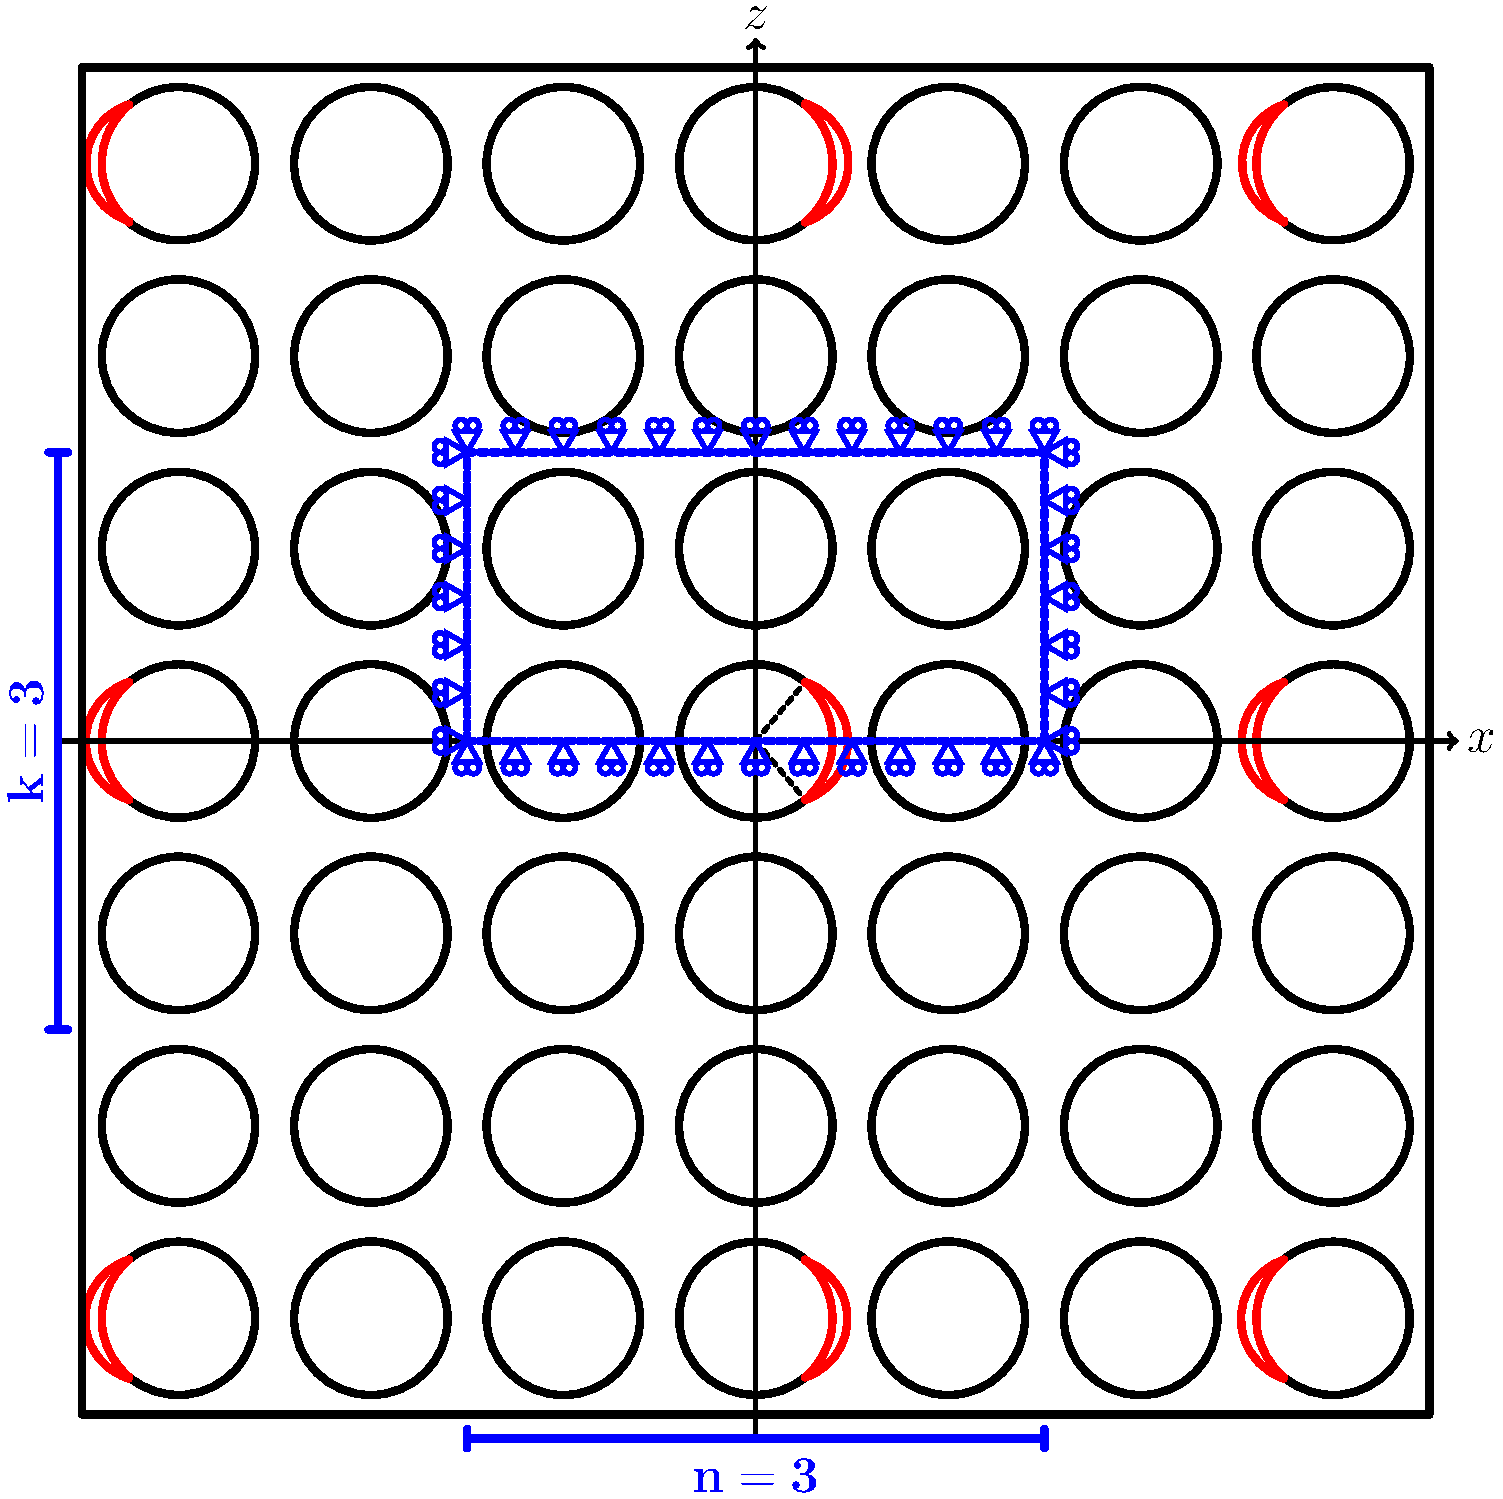
\includegraphics[width=\textwidth]{coupling.pdf}
\caption{Representative Volume Element $n\times k-symm$ of a UD composite with debonds appearing after $n-1$ and after $k-1$ undamaged fibers respectively in the horizontal and vertical direction. In the vertical direction, on fibers belonging to the same ``column'', debonds are located always on the same side.}\label{fig:laminateModelsA}
\end{figure}

In order to facilitate the description of the models, let us assume that the UD composite mid-plane lies in the $x-y$ plane, where $y$ coincides with the UD $0^{\circ}$ direction while the $x-axis$ represents the UD in-plane transverse direction. Axis $z$ is the through-the-thickness direction of the composite.

\begin{figure}[!h]
\centering
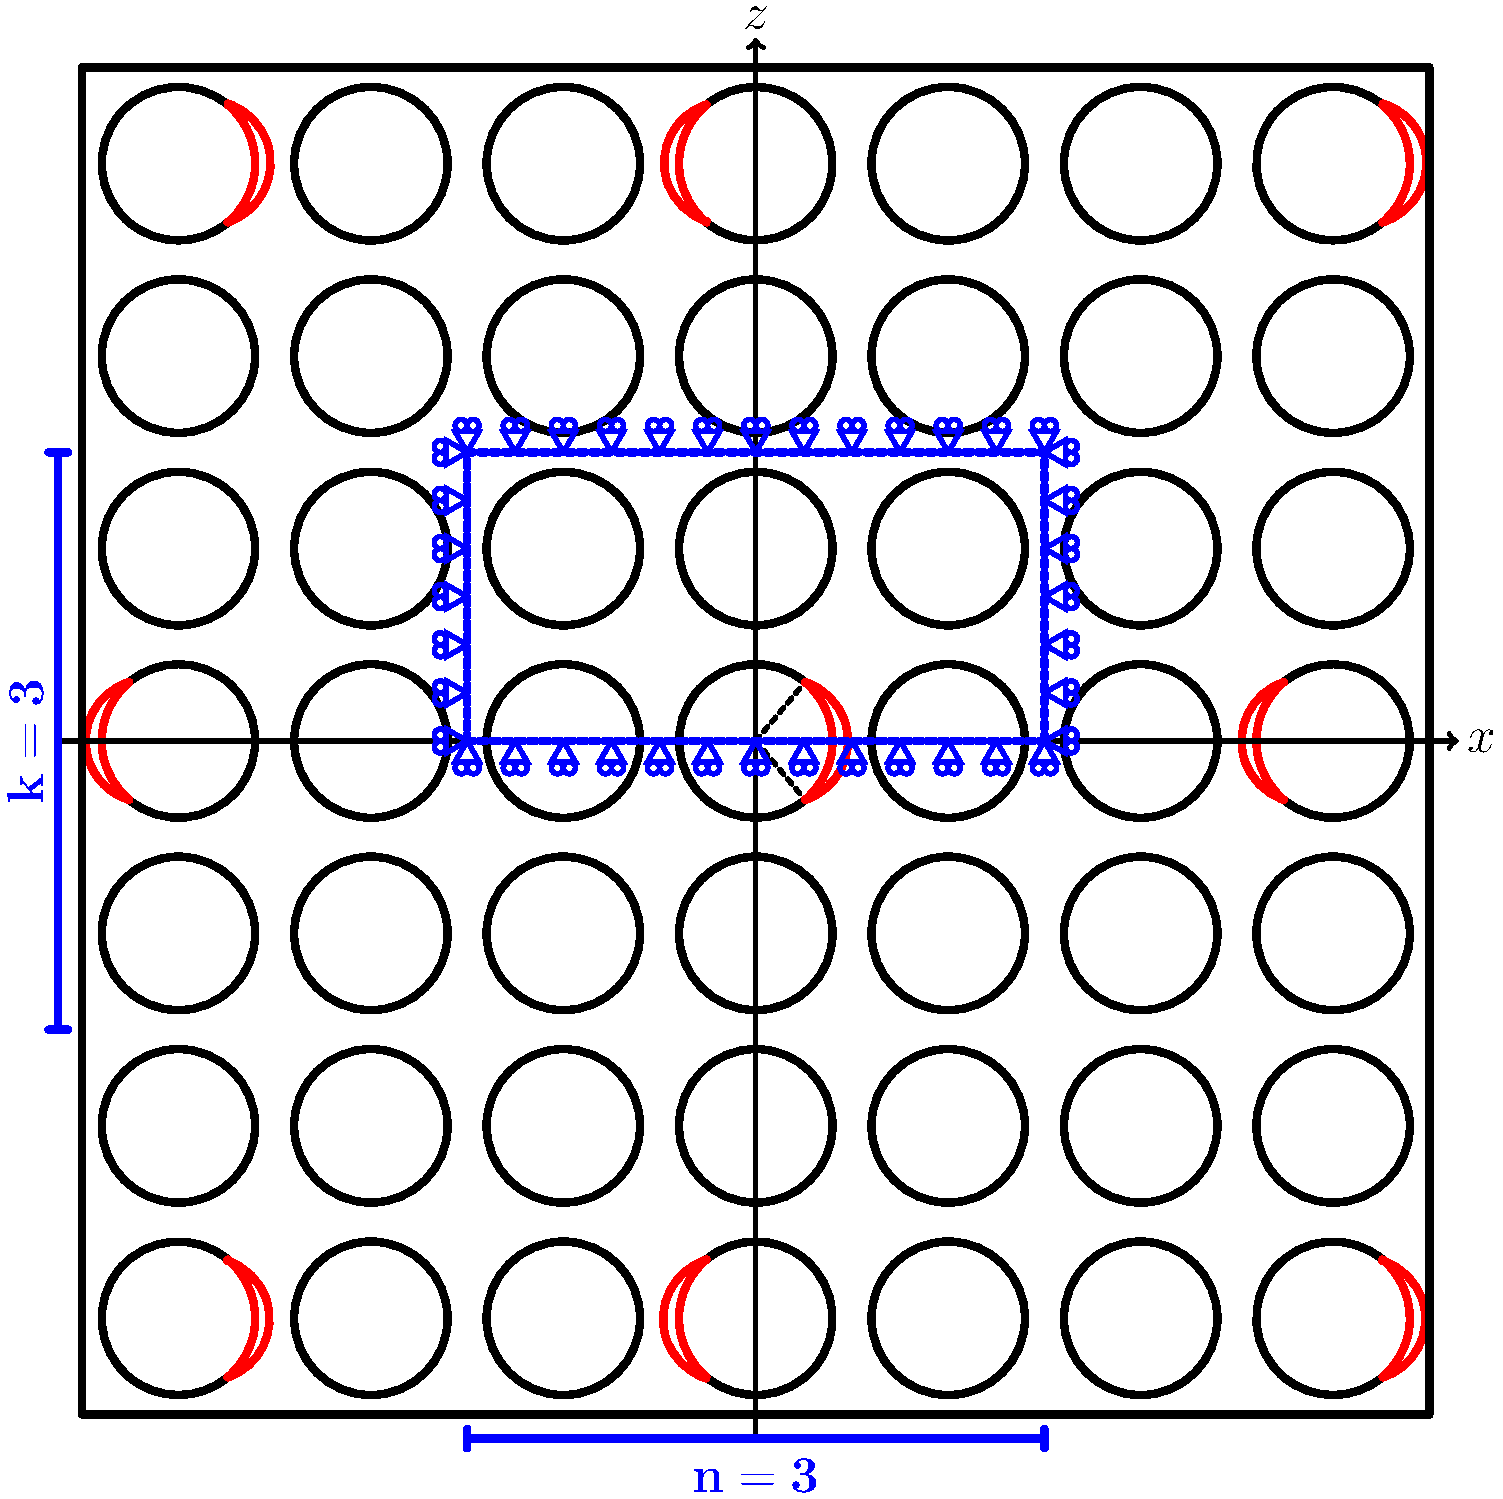
\includegraphics[width=\textwidth]{asymm.pdf}
\caption{Representative Volume Element $n\times k-asymm$  of a UD composite with debonds appearing after $n-1$ and after $k-1$ undamaged fibers respectively in the horizontal and vertical direction. In the vertical direction, on fibers belonging to the same ``column'', debonds are located on the opposite sides of consecutive fibers.}\label{fig:laminateModelsB}
\end{figure}

The composite RVE is defined in the $x-z$ plane and is repeating both along $x$ and $z$. Mathematically, it corresponds to an infinite UD composite which models, practically, the behavior of debonds located far away from the laminate free surfaces. i.e. close to the laminate mid-plane, in a relatively thick UD composite (thickness $>100$ fiber diameters). The composite with debonds is modeled as a sequence of fiber rows with or without debonds stacked on each other in the vertical (through-the-thickness) direction. Notice that each row contains only one fiber in the vertical direction. A regular microstructure is adopted for all RVEs, with fibers organized in a square-packing configuration. This choice is motivated by our interest in investigating the mechanisms that favors or prevent debond growth, and not in simulating crack path evolution in an arbitrary, randomized distribution of fibers. The regularity of the square-packing arrangement allows the identification of the different mechanisms influencing debond growth. Given their square-packing arrangement of fibers, each RVE is built by using the unit cell in Figure~\ref{fig:modelschem} as the basic building block. The unit cell contains one fiber place in its center and has a size of $2L\times2L$, where

\begin{equation}\label{eq:LVf}
L=\frac{R_{f}}{2}\sqrt{\frac{\pi}{V_{f}}}.
\end{equation}

In Equation~\ref{eq:LVf}, $V_{f}$ is the fiber volume fraction and $R_{f}$ the fiber radius. The fiber volume fraction is assumed equal to $60\%$ in each RVE and the fiber radius equal to $1\mu m$. The choice of the previous value is not dictated by physical considerations but by simplicity. It is thus useful to remark here that, in a linear elastic solution as the one considered in the present work, the ERR is proportional to the geometrical dimensions of the model and, consequently, recalculation of the ERR for fibers of any size requires a simple multiplication. Notice also that, given the relationship in Eq.~\ref{eq:LVf} and that the unit cell is identically repeated following a square-packing configuration, $V_{f}$ is homogeneous, i.e. no clustering of fibers is considered.

\begin{figure}[!h]
\centering
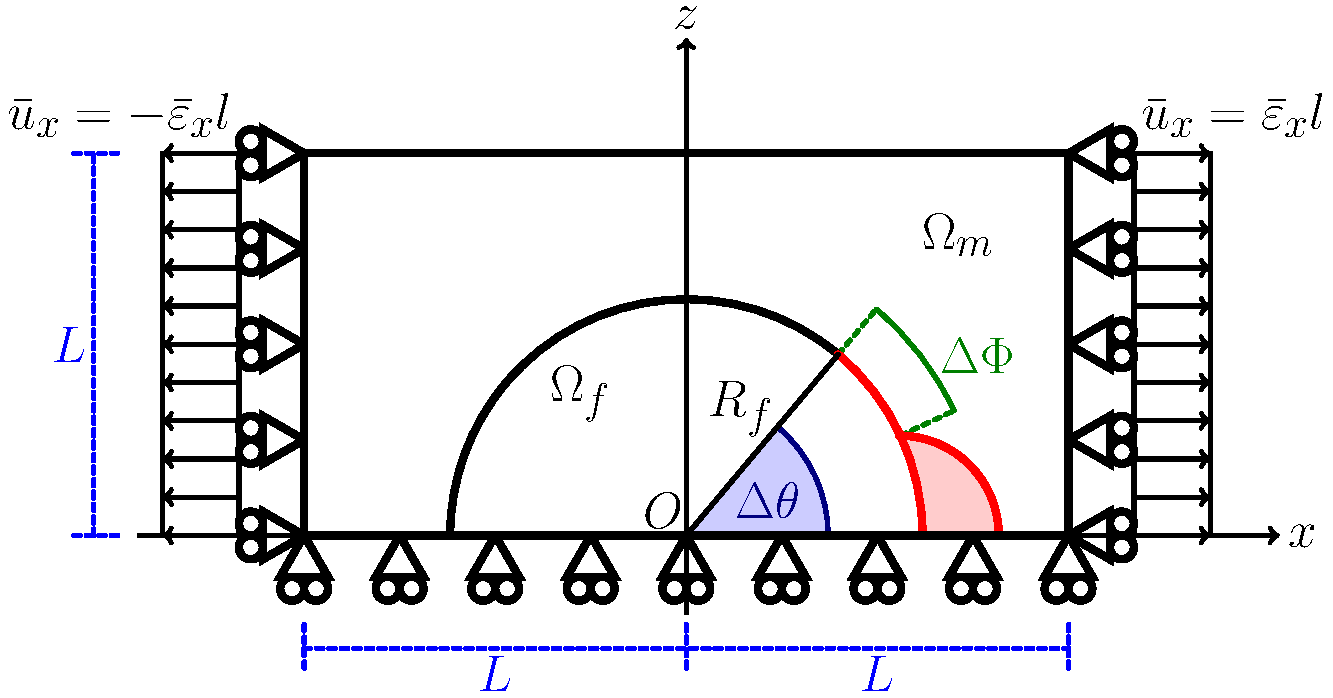
\includegraphics[width=\textwidth]{RUC.pdf}
\caption{Schematic of the model with its main parameters.}\label{fig:modelschem}
\end{figure}

A glass fiber-epoxy UD composite is treated in the present work, and it is assumed that the response of each phase lies always in the linear elastic domain. The material properties of glass fiber and epoxy are reported in Table~\ref{tab:phaseprop}.

\begin{table}[!htbp]
 \centering
 \caption{Summary of the mechanical properties of fiber and matrix. $E$ stands for Young's modulus, $\mu$ for shear modulus and $\nu$ for Poisson's ratio.}
 \begin{tabular}{cccc}
\textbf{Material} & \textbf{$E\left[GPa\right]$}\ & \textbf{$\mu\left[GPa\right]$} & \textbf{$\nu\left[-\right]$} \\
\midrule
Glass fiber    & 70.0  & 29.2   & 0.2  \\
Epoxy    & 3.5    & 1.25   & 0.4
\end{tabular}
\label{tab:phaseprop}
\end{table}

We consider that upon application of a load in the $x$-direction, the strain response in the $y$-direction is small due to the very small minor Poisson's ratio of the UD composite. We also assume that debond size to be significantly larger in the fiber longitudinal direction than in the arc direction. We therefore use 2D models under the assumption of plane strain defined in the $x-z$ section of the composite, which allows us to focus our interest on debond growth along the arc direction. Assumptions of generalized plane strain would be more suited to represent the physics, however it would limit the scope of comparisons with previous studies in the literature. It is for this reason that plane strain conditions are preferred.\\
All RVEs are symmetric with respect to the horizontal direction, thus only half of the RVE is explicitly modeled and symmetry conditions are applied to the lower boundary of the RVE (Fig.~\ref{fig:laminateModelsA} and Fig.~\ref{fig:laminateModelsB}). The number $n$ of fibers in the horizontal directions and $k$ in the vertical direction belonging to the RVEdetermine the total size of the RVE, described by its total length $l$ and total height $h$:

\begin{equation}\label{eq:lengthheight}
l=n2L\qquad h=k2L;
\end{equation}

where $2L$ is the side length of the square unit cell previously introduced and $L$ is defined according to Eq.~\ref{eq:LVf}. The number of fibers in the horizontal and vertical directions determine as well the damage state of the modeled UD composite. In particular, a $n\times k$ RVE represents a UD composite in which a debond appear after $n-1$ fully bonded fibers inside a fiber row, and a fiber row contains debonds after $k-1$ fiber rows with no damage (see Fig.~\ref{fig:laminateModelsA} and Fig.~\ref{fig:laminateModelsB}). To model such configurations, conditions of coupling of the horizontal displacement $u_{x}$ are applied to the right and left boundary, which ensures that the computed solution represents a model in which the RVE is repeated infinite times in the horizontal direction. It is worth to highlight that the repetition of the RVE occurs in a mirror-like fashion: moving along the $x$-axis, if a debond appears on the right side of its fiber, the next one is placed on the left side.\\
This might lead to extreme conditions in the model. Consider for example the case of $1\times k$ RVEs: inside a fiber row containing damage, an infinite number of debonds is present and debonds are facing each other pair-by-pair. Such configuration is physically unlikely, however the evaluation of the ERR in this case provides a bound for the case of maximum debond mutual interaction in the vertical direction. Thus, the models proposed here might represent extreme configuration, but they provide theoretical bounds for debond behavior in an actual composite. In particular, observations regarding mechanisms favoring debond growth will represent an upper bound on ERR and thus a conservative estimation of the actual behavior, still of use for the structural designer. Greater care should instead be taken when considering mechanisms preventing debond growth: the ERR estimate provided by our models would be a lower bound, thus debond growth might be higher than predicted in the actual composite.\\
Repetition occurs also along the vertical direction. Here two cases can be distinguished: first, debonds aligned in the vertical direction are placed on the same side of their respective fibers as in Figure~\ref{fig:laminateModelsA}; second; debonds aligned in the vertical direction are placed on alternating opposite sides of their respective fibers in Figure~\ref{fig:laminateModelsB}. The first is case of symmetric repetition with respect to the upper boundary of the RVE; the second case is one of anti-symmetric repetition with respect to the upper boundary of the RVE. The two different families of RVEs (symmetric with respect to anti-symmetric repetition) are thus respectively called $n\times k-symm$ and $n\times k-asymm$. The details of the boundary conditions adopted in the two different cases are described in Sec.~\ref{subsec:bc}.

\subsection{Equivalent boundary conditions: description and validation}\label{subsec:bc}

Two main families of Representative Volume Elements have been introduced in the previous section, distinguished by their pattern of repetition along the vertial direction: $n\times k-symm$ and $n\times k-asymm$.\\
To model the symmetric repetition of $n\times k-symm$ RVE ( Fig.~\ref{fig:laminateModelsA}) we adopt, on the upper boundary, conditions of coupling of the vertical displacements $u_{z}$ of the type

\begin{equation}\label{eq:symmcoupling}
u_{z}\left(x,h\right) = \bar{u}_{z},
\end{equation}

where $h$ is the total height of the RVE defined in Eq.~\ref{eq:lengthheight} and $\bar{u}_{z}$ is the constant value of the vertical displacement, equal for all the points on the upper boundary. The value of $\bar{u}_{z}$ is \emph{a priori} unknown and is evaluated as part of the elastic solution.\\
The asymmetric repetition of $n\times k-asymm$ RVE (Fig.~\ref{fig:laminateModelsB}) is modeled with the following set of conditions applied to the vertical $u_{z}$ and horizontal displacements $u_{x}$:

\begin{equation}\label{eq:asymmcoupling}
\begin{aligned}
u_{z}\left(x,h\right) - u_{z}\left(0,h\right) &= -\left(u_{z}\left(-x,h\right) - u_{z}\left(0,h\right)\right)\\
u_{x}\left(x,h\right) &= -u_{x}\left(-x,h\right),
\end{aligned}
\end{equation}

where $h$ is again the total height of the RVE and $u_{z}\left(0,h\right)$ is the vertical displacement of the upper boundary mid-point, which is always located at coordinates $(0,h)$. Similarly to $\bar{u}_{z}$ in the symmetric case, $u_{z}\left(0,h\right)$ is \emph{a priori} unknown and is computed as part of the elastic solution.

\begin{figure}[!h]
\centering
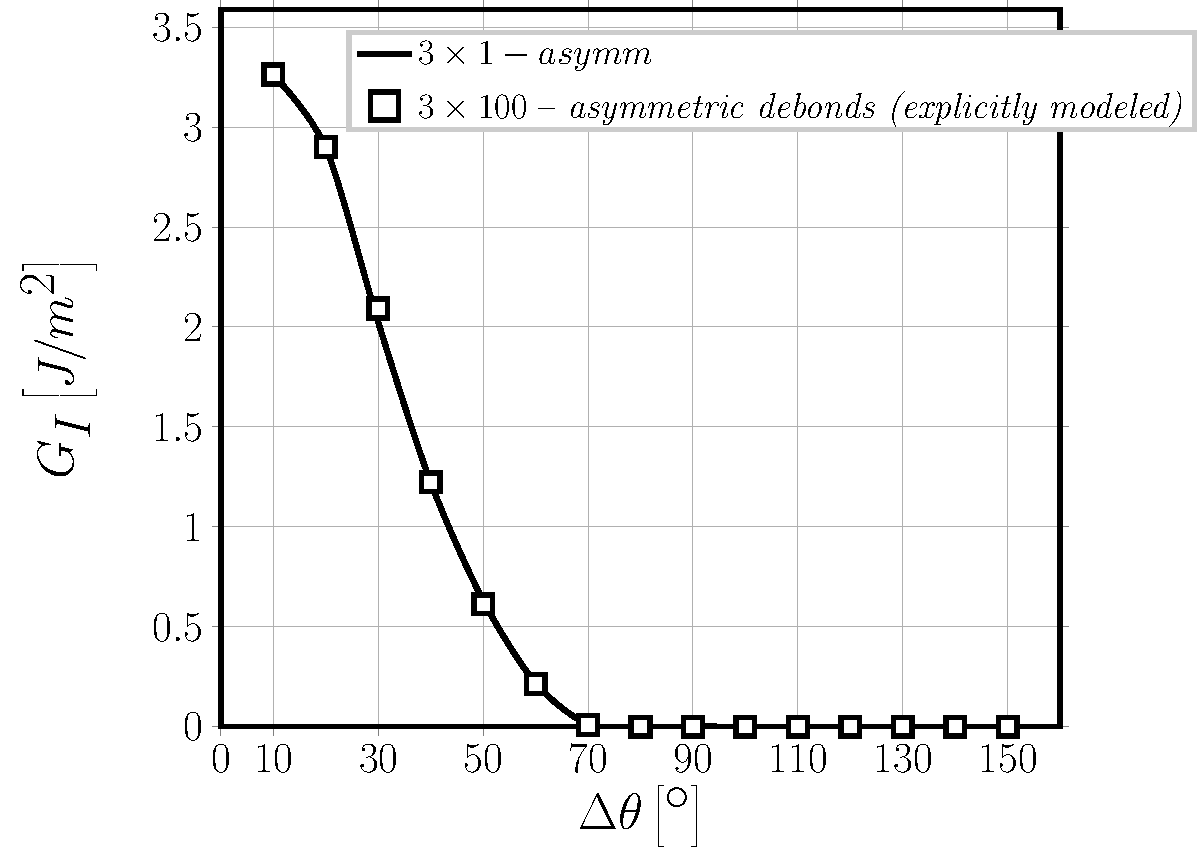
\includegraphics[width=\textwidth]{asymm-vs-explmodel-vf60-GI.pdf}
\caption{Validation of asymmetric coupling conditions of Eq.~\ref{eq:asymmcoupling}: Mode I ERR, $V_{f}=60\%$, $\bar{\varepsilon}_{x}=1\%$.}\label{fig:validationGI}
\end{figure}

To the authors' knowledge, this is the first time the set of boundary conditions of Eq.~\ref{eq:asymmcoupling} is proposed and used to model an asymmetric coupling as the one reported in Figure~\ref{fig:laminateModelsB}. To validate them, Mode I (Fig.~\ref{fig:validationGI}) and Mode II ERR (Fig.~\ref{fig:validationGII}) are evaluated for $3\times 1-asymm$ RVE and compared with the results of the $3\times100-asymmetric\ debonds\ (explicitly\ modeled)$ RVE, in the case of an applied strain $\bar{\varepsilon}_{x}$ of $1\%$. The $3\times201-asymmetric\ debonds\ (explicitly\ modeled)$ RVE possesses, as all other RVEs studied here, conditions of coupling of the horizontal displacement applied to the left and right side. It is as well symmetric with respect to the $x$-axis, thus only half of the RVE is modeled and conditions of symmetry are applied to the lower horizontal boundary. The upper side of the RVE is, differently from the other models studied here, left free. Debonds are explicitly modeled and placed on alternating sides of vertically aligned fibers, i.e. if a fiber has a debond on the right side the next fiber above will have the debond on the left side. Debonds are all of the same size. The $3\times201-asymmetric\ debonds\ (explicitly\ modeled)$ RVE thus represents the same configuration as the $3\times 1-asymm$ RVE, but explicitly modeled. Comparison of the ERR of the two RVEs provides a validation of accuracy of the conditions expressed in Eq.~\ref{eq:asymmcoupling} as a mean to represent the situation with alternating debonds (or asymmetric coupling, as depicted in Fig.~\ref{fig:laminateModelsB} with the use of equivalent boundary conditions, which is a more effective in terms of computational cost of the model (time and memory needed to compute the solution).

\begin{figure}[!h]
\centering
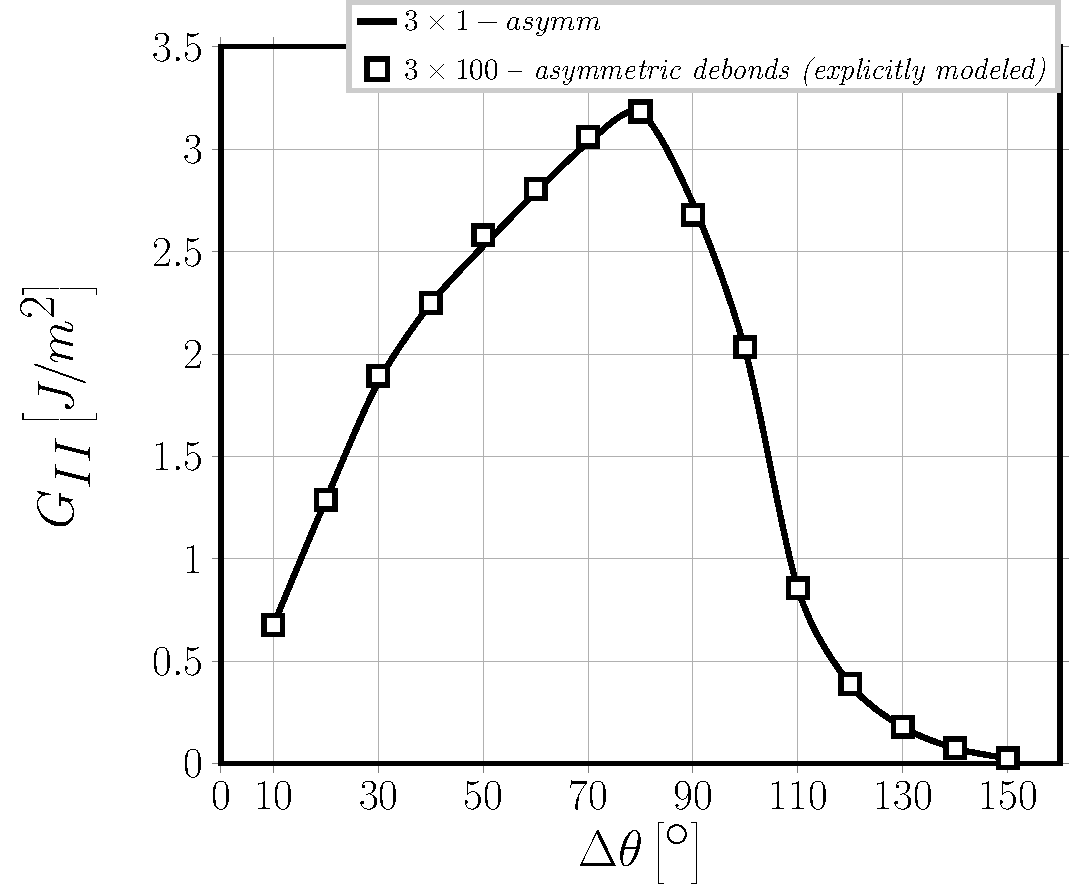
\includegraphics[width=\textwidth]{asymm-vs-explmodel-vf60-GII.pdf}
\caption{Validation of asymmetric coupling conditions of Eq.~\ref{eq:asymmcoupling}: Mode II ERR, $V_{f}=60\%$, $\bar{\varepsilon}_{x}=1\%$.}\label{fig:validationGII}
\end{figure}

As shown in Figure~\ref{fig:validationGI} and Figure~\ref{fig:validationGII}, a very good agreement is obtained between the results of the two RVEs for both Mode I and Mode II ERR. The validity of the asymmetric coupling conditions proposed in Equation~\ref{eq:asymmcoupling} is thus confirmed.

\subsection{Finite Element (FE) solution}

The solution of the elastic problem is obtained with the Finite Element Method (FEM) within the Abaqus environment, a commercial FEM software~\cite{abq12}.\\
The debond is placed symmetrically with respect to the $x$ axis (see Fig.~\ref{fig:modelschem}) and it is characterized by an angular size of $\Delta\theta$ (making the full debond size equal to $2\Delta\theta$). For large debond sizes (at least $\geq 60^{\circ}-80^{\circ}$), a region $\Delta\Phi$ of variable size appears at the crack tip where the crack faces are in contact but free to slide relatively to each other. In order to model crack faces motion in the contact zone, frictionless contact is considered between the two crack faces to allow free sliding and avoid interpenetration.\\
A constant displacement is applied to all RVEs, the magnitude of which is selected to have a constant applied horizontal strain $\bar{\varepsilon}_{x}$ equal to $1\%$. The choice of this specific value of the applied strain is actually arbitrary. In the context of Linear Elastic Fracture Mechanics, the Energy Release Rate at the debond tip is proportional to the square of the applied strain. Thus, ERR estimation at a different strain level requires a simple multiplication. Furthermore, our interest is to compare the effect of different mechanisms on debond growth, which we characterize with Mode I and Mode II ERR. As such, our focus is not on providing absolute values of ERR for specific damage configurations, but rather to assess and compare the relative changes in ERR due to modifications of the sorrounding environment. In this perspective, the selection of a rather large value of the applied strain helps our understanding by magnifying the differences in ERR. A further consideration regarding the magnitude of the load needs to be made, regarding the presence of contact between debond faces. The problem solved is a linear problem with non-holonomic constraints due to the non-interpenetration conditions (inequalities) enforced on crack faces relative displacements. In particular, the problem falls under the definition of receding contact problem~\cite{Paris1996,Garrido1991}. This family of problems in LEFM has some peculiar characteristics~\cite{Garrido1991,Keer1972,Tsai1974}: the size and shape of the contact zone does not depend on the magnitude of the applied load, but only on its type. Thus, upon a change in magnitude of the applied strain $\bar{\varepsilon}_{x}$ the size and shape of the contact zone at the fiber/matrix interface will remain the same.\\
Meshing of the model is accomplished with second order, 2D, plane strain triangular (CPE6, see~\cite{abq12}) and quadrilateral (CPE8, see~\cite{abq12}) elements. An oscillating singularity exists at the debond tip in the stress and displacement fields~\cite{England1971,Toya1974,Comninou1977}. The presence of this singularity prevents the convergence of Mode I and Mode II ERR at the debond tip. Thus, a correct Mode decomposition of the ERR can not be computed in the theoretical limit of an infinitesimal crack increment. It is possible however to avoid the issue by approximating the Mode decomposition over a finite instead of an infinitesimal crack increment. This leads naturally to the use of the Virtual Crack Closure Technique (VCCT)~\cite{Krueger2004}, which estimates Mode I and Mode II ERR over a finite crack increment corresponding to the size of the element at the crack tip. To obtain accurate results in terms of Mode decomposition of the ERR, care must be taken in ensuring the quality of the mesh at the debond tip. In particular, a regular mesh of 8-node ($2^{nd}$ order rectangular) elements with almost unitary aspect ratio is constructed at the debond tip. The angular size $\delta$ of an element in the debond tip neighborhood is always equal to $0.05^{\circ}$. The crack faces are modeled as element-based surfaces and a small-sliding contact pair interaction with no friction is imposed between them. The Mode I, Mode II and total Energy Release Rates (ERRs) (respectively referred to as $G_{I}$, $G_{II}$ and $G_{TOT}$) are the main result of FEM simulations; they are evaluated using the VCCT~\cite{Krueger2004} implemented in a in-house Python routine. Validation is performed with respect to the results reported in~\cite{Paris2007,Sandino2016}, which were obtained with the Boundary Element Method (BEM) for a model of a partially debonded single fiber placed in an infinite matrix. As discussed in more detail in~\cite{DiStasio2019}, the agreement between FEM (present work) and BEM~\cite{Paris2007,Sandino2016} solutions is good and the difference between the two does not exceed $5\%$. This provides us with a level of uncertainty with which we can analyze the significance of observed trends: any relative difference in ERR between different RVEs smaller than $5\%$ cannot be reliably distinguished from numerical uncertainty and its discussion should thus be avoided.

\section{Results \& Discussion}\label{sec:results}

\subsection{Interaction between isolated debonds in infinite UD composites}\label{subsec:chesstable}

The effect on Mode I and Mode II ERR of the interaction between debonds appearing at regular distances (in terms of fully bonded fibers) in the horizontal and vertical directions (models $n\times k-coupling$) is shown respectively in Figure~\ref{fig:debonddebondGI} and Figure~\ref{fig:debonddebondGII}. It can be observed that it is the distance between debonds in the horizontal direction that presents a relevant effect on ERR: the number of fully bonded fibers between consecutive debonds in the vertical direction has a negligible influence on Mode I and a very modest effect, below or at the limit of the $5\%$ accuracy of the model, on Mode II.

\begin{figure}[!h]
\centering
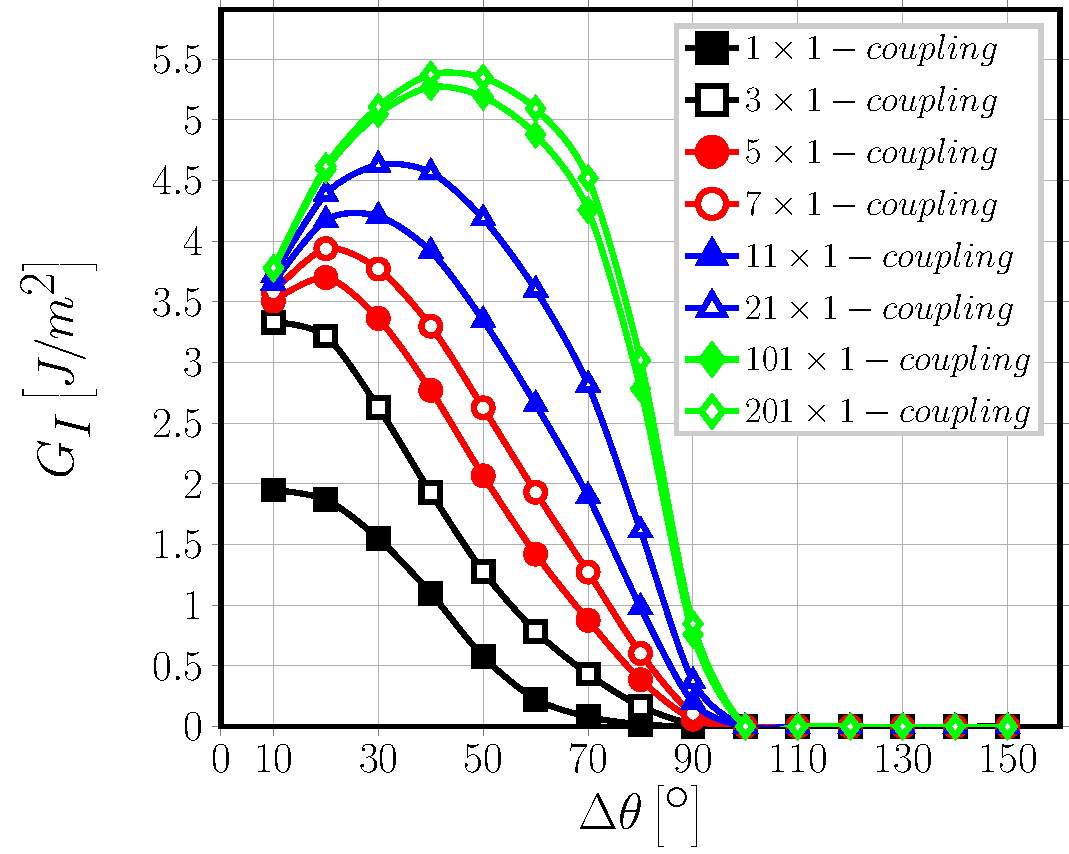
\includegraphics[width=\textwidth]{nx1-coupling-vf60-GI.pdf}
\caption{Effect of debond-debond interaction in infinite UD composites on Mode I ERR: models $n\times k-coupling$. $V_{f}=60\%$, $\varepsilon_{x}=1\%$.}\label{fig:nx1GI}
\end{figure}

On the other hand, increasing the number of fully bonded fibers between debonds in the horizontal direction leads to a significant increase in both Mode I and Mode II ERR, due to the magnification of the $x$-strain in the crack tip neighborhood~\cite{DiStasio2019}. A critical distance (in terms of undamaged fibers) at which a non-interacting solution can be observed is apparent for Mode I (Figure~\ref{fig:debonddebondGI}). Given that Mode II ERR for models $21\times 3-coupling$, $21\times 21-coupling$, $101\times 3-coupling$ and $101\times 101-coupling$ is in a $\leq5\%$ range with respect to each other and thus their difference is not significant taking into account model accuracy, it can be argued that also in Mode II a critical distance exists at which a non-interacting solution appears.

\begin{figure}[!h]
\centering
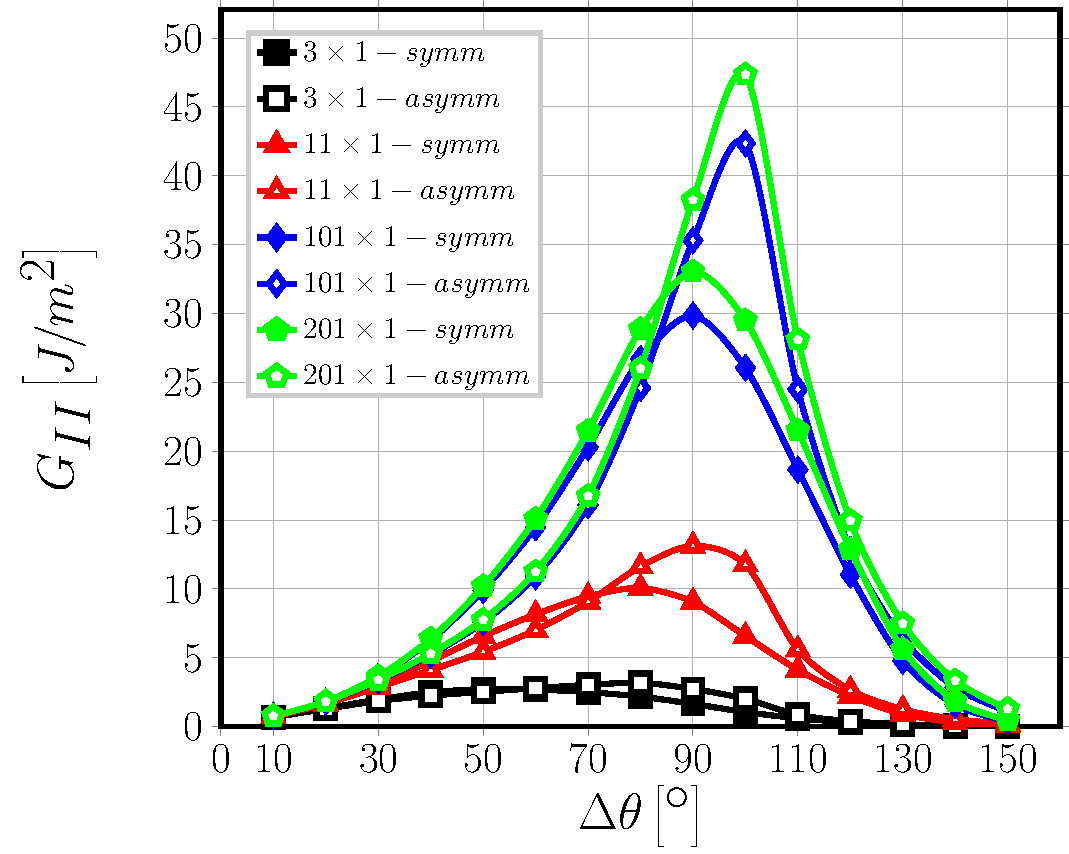
\includegraphics[width=\textwidth]{nx1-coupling-vf60-GII.pdf}
\caption{Effect of debond-debond interaction in infinite UD composites on Mode II ERR: models $n\times k-coupling$. $V_{f}=60\%$, $\varepsilon_{x}=1\%$.}\label{fig:nx1GII}
\end{figure}

\subsection{Debond-debond interaction between horizontal rows of partially debonded fibers in infinite UD composites}\label{subsec:horizontal}

The results presented in Figures~\ref{fig:horizontalGI} and~\ref{fig:horizontalGII} for respectively Mode I and Mode II ERR of models $1\times k-coupling$ confirm the observations presented in Section~\ref{subsec:chesstable}. Models $1\times k-coupling$ represents the RVE of an infinite UD composite with horizontal fiber rows that appear at regular intervals (measured in terms of fully bonded fibers) and in which fibers are all partially debonded (see Fig.~\ref{fig:laminateModelsC} for reference).

\begin{figure}[!h]
\centering
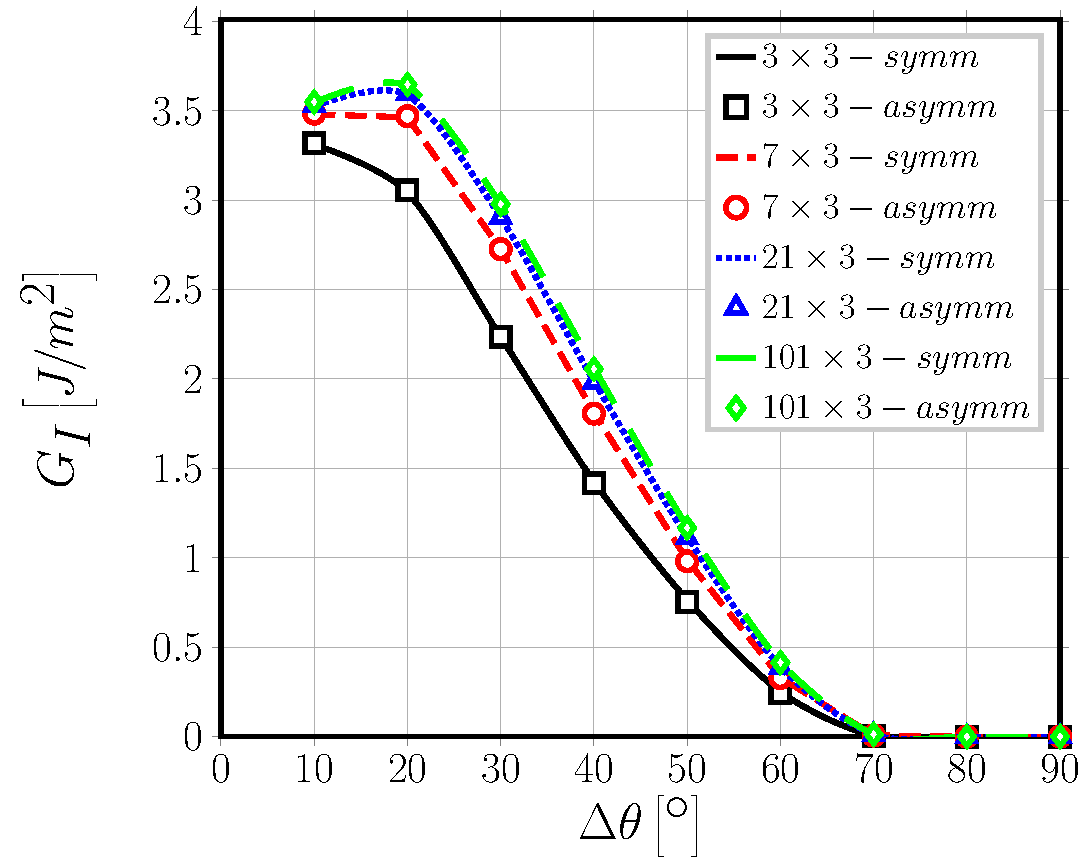
\includegraphics[width=\textwidth]{nxk-coupling-vf60-GI.pdf}
\caption{Effect of debond-debond interaction in infinite UD composites on Mode I ERR: models $1\times k-coupling$. $V_{f}=60\%$, $\varepsilon_{x}=1\%$.}\label{fig:nxkGI}
\end{figure}

Varying the number $k$ of undamaged fibers between fiber rows of only partially debonded fibers does not have any effect on ERR, neither in Mode I (Figure~\ref{fig:horizontalGI}) nor in Mode II (Figure~\ref{fig:horizontalGII}). The observations of Sec.~\ref{subsec:chesstable} are thus confirmed: it is the presence of fully bonded fibers only in the horizontal direction, i.e. the loading direction, that affects the debond ERR through $x$-strain magnification.

\begin{figure}[!h]
\centering
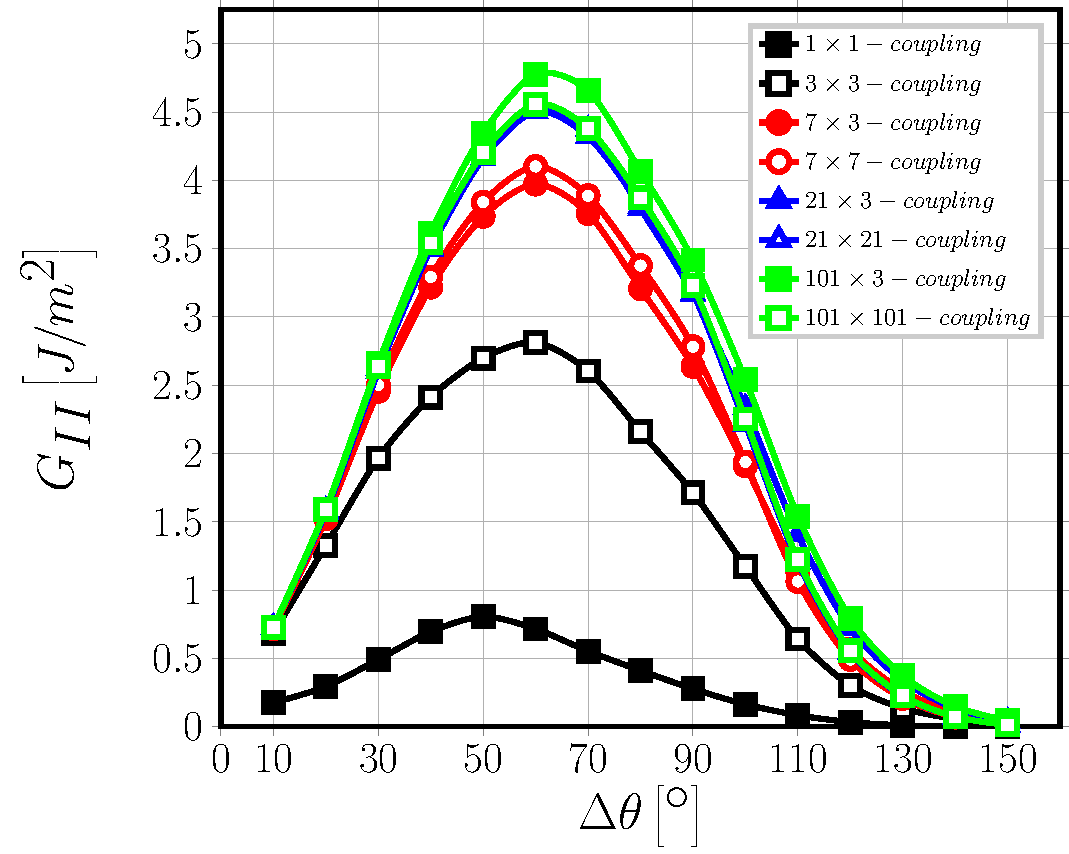
\includegraphics[width=\textwidth]{nxk-coupling-vf60-GII.pdf}
\caption{Effect of debond-debond interaction in infinite UD composites on Mode II ERR: models $1\times k-coupling$. $V_{f}=60\%$, $\varepsilon_{x}=1\%$.}\label{fig:nxkGII}
\end{figure}



\section{Conclusions}\label{sec:conclusions}

Different models of infinite UD composites have been studied with different configurations of multiple interacting debonds in order to investigate their effect of Mode I and Mode II Energy Release Rate.\\
Building upon the observations made in the previous section, several conclusions can be drawn about the growth of debonds in UD composites:

\begin{itemize}
\item at given strain level, multiple debonds can appear on not consecutive vertically-aligned fibers;
\item at a given strain level, the vertical lines of fibers on which debonds grow are determined by the horizontal distance from pre-existing debonds;
\item a minimum non-interactive distance exists for the Energy Release Rate;
\item when spacing between vertical lines of debonds is lower than the minimum non-interactive distance, the ERR decreases;
\item thus, conversely, when spacing between vertical lines of debonds is lower than the minimum non-interactive distance, higher levels of strain are needed to grow debonds;
\item growth of debonds appearing on contiguous vertically-aligned fibers is energetically the most favorable;
\item larger debonds are favored on contiguous vertically aligned partially debonded fibers.
\end{itemize}



\begin{acknowledgements}
Luca Di Stasio gratefully acknowledges the support of the European School of Materials (EUSMAT) through the DocMASE Doctoral Programme and the European Commission through the Erasmus Mundus Programme.
\end{acknowledgements}


% Authors must disclose all relationships or interests that 
% could have direct or potential influence or impart bias on 
% the work: 
%
% \section*{Conflict of interest}
%
% The authors declare that they have no conflict of interest.


% BibTeX users please use one of
%\bibliographystyle{spbasic}      % basic style, author-year citations
\bibliographystyle{spmpsci}      % mathematics and physical sciences
%\bibliographystyle{spphys}       % APS-like style for physics
\bibliography{refs}   % name your BibTeX data base

%% Non-BibTeX users please use
%\begin{thebibliography}{}
%%
%% and use \bibitem to create references. Consult the Instructions
%% for authors for reference list style.
%%
%\bibitem{RefJ}
%% Format for Journal Reference
%Author, Article title, Journal, Volume, page numbers (year)
%% Format for books
%\bibitem{RefB}
%Author, Book title, page numbers. Publisher, place (year)
%% etc
%\end{thebibliography}

\end{document}
% end of file template.tex

